Feedback-driven speech recognition uses generated text as input to later
inference. A trusted correction can change that input, invalidating some
speculative work while leaving other work usable. A dependable service
must distinguish these cases and preserve useful delivered progress while
the trusted path catches up.

Computation retention alone can exacerbate this mismatch. In our
predeclared Qwen evaluation on three new eight-speaker cohorts, retaining
valid computation improved timely delivery but increased observed
audio-frontier withdrawals from 12 to 17 when the Consumer still installed
snapshots. Retaining the computation and its compatible whole view together
produced zero frontier withdrawals in that stratum. The issue is how valid
work becomes sustained service across a trusted update.

One actual two-second interval illustrates the loss. Its complete
hypothesis reached the Consumer at 1.444~s, meeting the two-second display
deadline. At 1.544~s, a new certified root replaced it with a shorter
snapshot, although the whole hypothesis retained a valid dependency path.
It remained absent at the original deadline and returned with identical
text at 3.720~s through certified delivery, within the eight-second deadline.
Both first-delivery obligations were met, yet 37 newly displayed characters,
including spaces, disappeared for 2.176~s. This is lost interval coverage
under a compatible update, independently of transcription correctness.

\begin{figure*}[t]
\centering
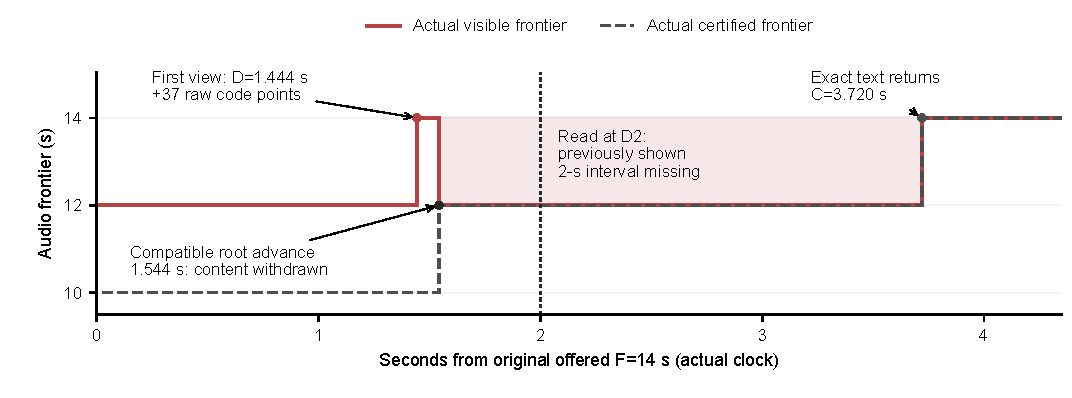
\includegraphics[width=\textwidth]{figures/timely_full_interval_case.pdf}
\caption{An actual computation-only interval meets first-display D2 and
certified-delivery C8, yet loses its phrase for 2.176~s under a compatible
update. The dotted line samples the original D2 read point. This case
comes from c16, whose whole-run D2 P99 fails; it is neither a paired
counterfactual nor a natural-prevalence estimate.}
\label{fig:continuity_case}
\end{figure*}

Incremental dialogue distinguishes active and committed information and
propagates revocation~\cite{schlangen2011incremental}; incremental
computation reuses dependencies and stable identities
\cite{hammer2014adapton,hammer2015names,mcsherry2013differential}.
SSBD combines old draft reuse with display-only masking in
re-translation~\cite{zeng2026ssbd}, and PredGen speculates on downstream
responses during evolving speech~\cite{li2025predgen}. RevTrace applies
these ideas to a protected task whose original selection recursively
supplies later ASR inputs. Separate sufficient guards determine whether
old computation remains eligible and whether installing a root preserves
the Consumer's current whole hypothesis. Original selection retains
write authority and incompatible revisions remain necessary.

Complete frozen inputs supply the eligibility witness. The core runtime
checks recorded continuation paths; a native correction pipeline confirms
inputs of already executing full calls. A call can have a valid input
even when its own predicted next state is wrong. The Consumer independently
checks its visible whole view. Selected facts, provisional views, and
physical execution retain distinct identities through message rejection,
durable selection, and recovery.

This paper makes three contributions:
\begin{itemize}
\item A feedback-state contract with separate executable witnesses for
  computation eligibility and whole-view retention across selected roots.
  Complete inputs, output dependencies, and execution identities determine
  what survives; a version change alone does not.
\item A coordinator that preserves the original selected transition relation
  while retaining compatible computation and views. Its conditional
  guarantees distinguish provisional delivery, durable selection, and
  physical ownership, including supported process failures.
\item Actual service evidence with the selected task fixed: factorial
  controls expose computation-only withdrawal, native correction tests
  input-confirmed full calls, and fault and sustained-state trials test
  the coordinator's boundaries and costs.
\end{itemize}

The headline joint design adds 26.645~s of dual-deadline credit over
714.110~s offered without changing certified histories. A separate 48-run
study retains the negative intermediate-load result and distinguishes
subsequent availability from first delivery. Earlier native confirmation
on four new speakers raises credit from 37.0 to all 66.340~s offered
and whole-run D2/C8 passes from zero to eight of eight runs.
